\documentclass[12pt,a4paper]{article}

\usepackage{composites2019}

%% Numbered
%\bibliographystyle{model1-num-names}

%% Numbered without titles
%\bibliographystyle{model1a-num-names}

%% Harvard
%\bibliographystyle{model2-names.bst}\biboptions{authoryear}

%% Vancouver numbered
%\usepackage{numcompress}\bibliographystyle{model3-num-names}

%% Vancouver name/year
%\usepackage{numcompress}\bibliographystyle{model4-names}\biboptions{authoryear}

%% APA style
%\bibliographystyle{model5-names}\biboptions{authoryear}

%% AMA style
%\usepackage{numcompress}\bibliographystyle{model6-num-names}

%% `Elsevier LaTeX' style
%\bibliographystyle{elsarticle-num}
%%%%%%%%%%%%%%%%%%%%%%%

\begin{document}
\thispagestyle{empty}

\vspace*{-3.4cm}
\begin{table}[!h]
\begin{tabular}{r}
\hspace*{2.9cm} \scriptsize \textsf{7th ECCOMAS Thematic Conference on the Mechanical Response of Composites: COMPOSITES 2019} \\
\hspace*{2.9cm} \tiny \textsf{A. Turon, P. Maimí \& M. Fagerström (Editors)}
\end{tabular}
\end{table}

\vspace*{-0.7cm}

\begin{center}
\title{ESTIMATING THE AVERAGE SIZE OF FIBER/MATRIX INTERFACE CRACKS IN UD AND CROSS-PLY LAMINATES}
\end{center}
\begin{center}
\textbf{\underline{Luca Di Stasio}$^{1,2,*}$, Janis Varna$^{2}$, Zoubir Ayadi$^{1}$} \\ [7pt]
\small{$^1$~Universit\'e de Lorraine, EEIGM, IJL, 6 Rue Bastien Lepage, F-54010 Nancy, France}  \\  [2pt]
\small{$^2$~Lule\aa\ University of Technology, University Campus, SE-97187 Lule\aa, Sweden}  \\  [2pt]
\small{$^*$~\texttt{luca.di.stasio@ltu.se}} \\
\end{center}

\noindent
%Onset of transverse cracking manifests itself at first in the form of fiber/matrix interface cracks (debonds), that propagate along the arc direction of the fiber surface and coalesce together to form a continuous through-the-ply thickness crack. 
Characterization of fiber/matrix interface cracks (debonds) has mainly focused on the evaluation of the Energy Release Rate (ERR). However, the attention has been mostly devoted to the study of a single partially debonded fiber placed in an effectively infinite medium and to the effect of a small number of nearby fibers on debond ERR~\cite{Sandino2016}. In this work, the Mode I and Mode II ERRs are evaluated for debonds appearing in Representative Volume Elements (RVEs) of regular microstructures of UD (Fig.~\ref{fig:sizeesti}) and cross-ply laminates. By adopting a 2-parameters energy-based criterion for propagation~\cite{Hutchinson1992}, we then proceed to the estimation of the expected average debond size in different microstructural arrangements (see Fig.~\ref{fig:sizeesti}). Finally, the results are compared with available microscopic observations~\cite{Correa2018}.

\begin{figure}[h]
\centering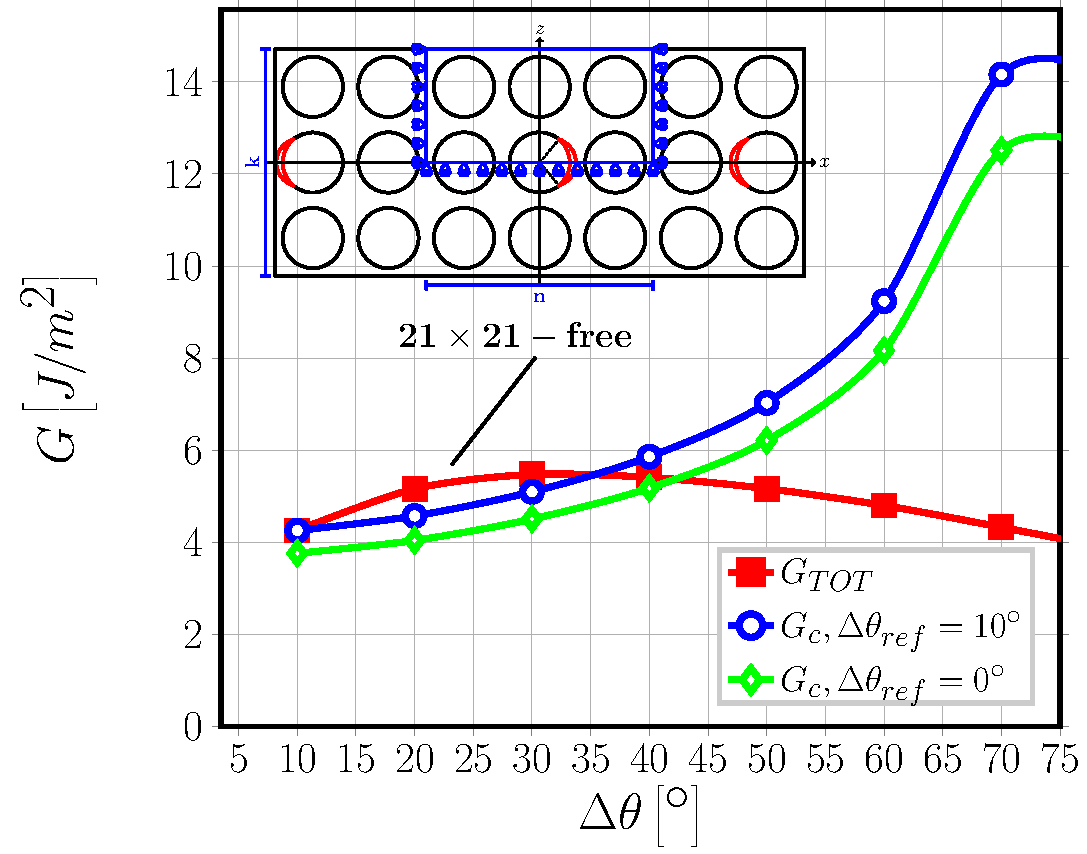
\includegraphics[width=0.551\textwidth]{vf60-GTOT.pdf}
\caption{Estimation of debond size by comparing the total ERR to the 2-parameters expression of critical $G_{c}$. Glass fiber/epoxy, $V_{f}=60\%$, $\varepsilon_{x}=1\%$.}
\label{fig:sizeesti}
\end{figure}

\begin{thebibliography}{9}
%
%% === Replace this by your references ===
%
\bibitem{Sandino2016} C. Sandino, E. Correa and F. Par{\'{\i}}s (2016) Numerical analysis of the influence of a nearby fibre on the interface crack growth in composites under transverse tensile load. \textit{Engineering Fracture Mechanics}, \textbf{168}, 58--75.
\bibitem{Hutchinson1992} J.W. Hutchinson and Z. Suo (1992) Mixed mode cracking in layered materials. J.W. Hutchinson, T.Y. Wu (Eds.), \textit{Advances in applied mechanics}, \textbf{29}, 63-191, Academic Press, New York.
\bibitem{Correa2018} E. Correa, M. I. Valverde, M .L. Velasco and F. París (2018) Microscopical observations of inter-fibre failure under tension. \textit{Engineering Fracture Mechanics}, \textbf{155}, 213--220.
%\bibitem{Pimenta} S. Pimenta and S.T. Pinho (2012) The effect of recycling on the mechanical response of carbon fibres and their composites. \textit{Composite Structures}, \textbf{94}, 3669-3684.
%
\end{thebibliography}

\end{document}
  
